% !BIB program = biber
\providecommand{\topdir}{../..} 
\documentclass[\topdir/lecture\_notes.tex]{subfiles}
\graphicspath{{\subfix{./images/}}}

\begin{document}
\section{The Solow-Swan Model}

The first growth model compatible with the stylized Kaldor facts was developed independently by Solow and Swan.
The central element of their theory is the notion of an aggregate production function:
\begin{equation}
  Y(t)=F(K(t), L(t), t) \label{eq:solow-production-function}
\end{equation}
where $Y$ is aggregate output, $K$ is the aggregate capital stock, $L$ is aggregate employment, and $t$ is the time index that appears separately in the production function to indicate that other factors such as technology may not be constant over time.
We assume that the production function has constant returns to scale
\begin{equation}
  F(\lambda K(t), \lambda L(t), t)=\lambda F(K(t), L(t), t), \quad \text { for } \lambda>0. \label{eq:solow-constant-returns}
\end{equation}

Aggregate saving in the economy is assumed to be a constant fraction of output
\begin{equation}
  S(t)=s Y(t), \quad 0<s<1, \label{eq:solow-savings}
\end{equation}
where $s$ is the constant propensity to save out of income (recall output and income are the same in aggregate).
We assume a closed economy with no government purchases of goods and services, and therefore
\begin{equation}
  Y(t)=C(t)+I(t), \label{eq:solow-output-identity}
\end{equation}
where $C$ is consumption of the representative household and $I$ is aggregate investment.
Equations \eqref{eq:solow-savings} and \eqref{eq:solow-output-identity} imply that consumption is also a constant fraction of output
\begin{equation}
  C(t)= (1-s) Y(t). \label{eq:solow-consumption}
\end{equation}

The change in capital over time is given by investment net of depreciation:
\begin{equation}
  \dot{K}(t)=I(t)-\delta K(t), \label{eq:solow-capital-accumulation}
\end{equation}
where $\delta>0$ is the constant depreciation rate and $\dot{K}(t) := dK(t) / dt$.

The labor force grows at a constant rate $n$:
\begin{equation}
  \dot{L}(t)=n L(t), \label{eq:solow-labor-growth}
\end{equation}
where $\dot{L}(t) := dL(t) / dt$, and $L(t_{0})$ is the initial level.
We assume that population grows at the same rate as the labor force, so ``per worker'' and ``per capita'' are the same in this model.

\subsection{No technological progress}
We first look at the case in which the production function does not directly depend on time:
\begin{equation}
  Y(t)=F(K(t), L(t)). \label{eq:solow-production-no-tech}
\end{equation}
Since $Y(t)$ can only depend on $t$ through $K(t)$ or $L(t)$, the production function \eqref{eq:solow-production-function} does not allow for technological progress.

In addition to constant returns to scale, we assume that the production function has positive but diminishing marginal products to both factors:
\begin{equation}
  F_{K}, F_{L}>0, \quad F_{K K}, F_{L L}<0, \quad F_{K L}>0. \label{eq:solow-marginal-products}
\end{equation}
These properties and constant returns to scale imply that $F_{K L}>0$.

A more controversial assumption, but one we will make nonetheless, is that $F(\cdot)$ obeys the so-called Inada conditions (after \parencite{inada1963conditions})
\begin{equation}
  \lim _{K \rightarrow 0} F_{K}=\lim _{L \rightarrow 0} F_{L}=+\infty, \quad \lim _{K \rightarrow \infty} F_{K}=\lim _{L \rightarrow \infty} F_{L}=0. \label{eq:solow-inada-conditions}
\end{equation}
These conditions are not innocuous and preclude a number of interesting non--standard cases.

The Solow-Swan model consists of equations \eqref{eq:solow-constant-returns}-\eqref{eq:solow-inada-conditions}.

It is convenient to write the model in per--worker terms, also called \new{intensive form}.
Define
\begin{align*}
  y(t) &:= \frac{Y(t)}{L(t)}, \\
  k(t) &:= \frac{K(t)}{L(t)}, \\
  c(t) &:= \frac{C(t)}{L(t)}.
\end{align*}

Dividing both sides of \eqref{eq:solow-production-no-tech} by $L(t)$ and using \eqref{eq:solow-constant-returns} with $\lambda = 1/L$, we get
\begin{equation}
  \frac{Y(t)}{L(t)} = \frac{1}{L(t)} F(K(t), L(t)) = F \left(\frac{K(t)}{L(t)}, 1\right). \label{eq:solow-output-per-worker}
\end{equation}
We define the intensive form of the production function
\begin{equation}
  f(k(t)) := F \left(\frac{K(t)}{L(t)}, 1\right). \label{eq:solow-intensive-production}
\end{equation}
and write \eqref{eq:solow-output-per-worker} as
\begin{equation}
  y(t) = f(k(t)). \label{eq:solow-intensive-form}
\end{equation}
The properties of $F$ imply the corresponding properties for $f$:
\begin{equation}
  f(0)=0 ; \quad f^{\prime}(k)>0 ; \quad f^{\prime \prime}(k)<0.
\end{equation}

Using the definition of $k(t)$, the chain rule, and \eqref{eq:solow-labor-growth}, we get
\begin{align}
\dot{k}(t) & = \frac{1}{L(t)} \cdot \dot{K}(t)-\frac{K(t)}{L(t)^{2}} \cdot \dot{L}(t) \\
           & =\frac{\dot{K}(t)}{L(t)}-n k(t).
           \label{eq:solow-k-dot-derivation}
\end{align}

Equations \eqref{eq:solow-savings}-\eqref{eq:solow-consumption} imply that $S=I$.
Combining $S=I$, \eqref{eq:solow-savings}, and \eqref{eq:solow-capital-accumulation} gives
\begin{equation}
  \dot{K}(t)=s Y(t)-\delta K(t) \label{eq:solow-capital-dot}
\end{equation}
Dividing by $L(t)$ and using \eqref{eq:solow-capital-dot} and \eqref{eq:solow-intensive-form}, we arrive at
\begin{equation}
  \dot{k}(t)=s f(k(t))-\left(\delta+n\right) k(t). \label{eq:solow-fundamental-equation}
\end{equation}

Equation \eqref{eq:solow-fundamental-equation} is the central equation of the Solow-Swan model.
If we understand and solve this central equation, we can understand and solve the rest of the model fairly straightforwardly.

\subsection{Equilibrium}
Figure~\ref{fig:solow-neoclassical-growth} shows a diagram of the $\dot{k}(t)$--equation.
The vertical axis shows levels whereas the horizontal axis shows capital per unit of effective labor, $k(t)$.

\begin{figure}[h]
\begin{center}
 %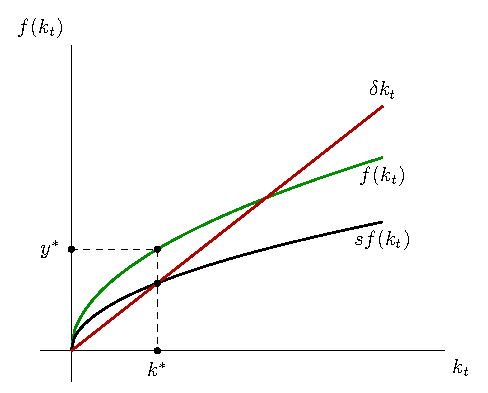
\includegraphics[width=0.75\textwidth]{solow_neoclassical_growth}
 \caption{The neoclassical growth diagram}
 \label{fig:solow-neoclassical-growth}
\end{center}
\end{figure}

The two most important lines here are the

The curve $s f(k(t))$ represents the actual investment; it is concave since $f^{\prime \prime}(k(t))<0$.
The line $(\delta+n) k(t)$ is referred to as the break-even level of investment.
Beyond these curves, however, there is also the $f(k(t))$ curve.
Note that the vertical distance between the $s f(k(t))$ and $f(k(t))$ curves equals $c(t)=C(t) / L(t)$, i.e. consumption per unit of labor.

At low levels of $k(t)$, $\dot{k}(t)>0$, whereas at high levels of $k(t)$, $\dot{k}(t)<0$.
The only steady--state for $k(t)$ in Figure~\ref{fig:solow-neoclassical-growth} occurs at $k^{*}$, which is defined by the point where the curve $s f(k(t))$ and the line $(\delta+n) k(t)$ intersect.
At $k^{*}$, actual investment and breakeven investment are equal so capital per capita remains constant, $\dot{k}(t)=0$.
When $\dot{k}(t)=0$, $k(t)$ is constant, which implies that $K(t)$ and $L(t)$ grow at a ``balanced'' rate.

\subsection{Implications}
\subsection{Cobb-Douglas functional form}
If we assume a Cobb-Douglas functional form for the production function $F(K(t), L(t)) = K(t)^{\alpha} L(t)^{1-\alpha}$, we will have the following $\dot{k}(t)$-equation:

\begin{equation}
  \dot{k}(t)=s k(t)^{\alpha}-(\delta+n) k(t) \label{eq:solow-k-dot-cobb-douglas}
\end{equation}

From this expression, we can also derive the growth rate per worker (by using the chain rule):

\begin{equation}
\begin{aligned}
\frac{\dot{y}(t)}{y(t)} & =\frac{\frac{\partial\left(k(t)^{\alpha}\right)}{\partial t}}{k(t)^{\alpha}}=\frac{\alpha k(t)^{\alpha-1} \dot{k}(t)}{k(t)^{\alpha}}=\frac{\alpha \dot{k}(t)}{k(t)} \\
& =s \alpha k(t)^{\alpha-1}-\alpha(\delta+n)=\frac{s \alpha}{k(t)^{1-\alpha}}-\alpha(\delta+n)
\end{aligned}
\label{eq:solow-growth-rate-per-worker}
\end{equation}

\begin{figure}[h]
\begin{center}
  % 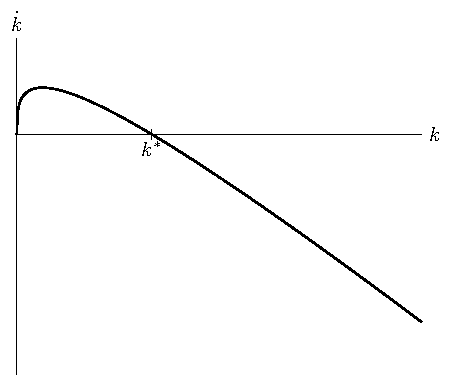
\includegraphics[width=0.75\textwidth]{solow_kdot}
  \caption{Impact on growth rate per worker of an increase in the savings rate}
  \label{fig:solow-savings-impact}
\end{center}
\end{figure}

In the short run, the growth rate depends on the initial capital per worker $k(t)$.
Economies that begin with low $k(t)$ have $\dot{k}(t)>0$ and grow faster; as $k(t)$ rises, the economy converges toward the steady state $k^{*}$ where $\dot{k}(t)=0$.
Starting from $k^{*}$, a permanent increase in the saving rate $s$ changes the steady state.
The new steady state $k^{**}$ is higher than $k^{*}$.
Just after the change in $s$, the economy is now below its steady-state.
This implies that $\dot{k}(t)>0$, temporarily lifting the growth rate.
Once $k(t)$ reaches the new, higher steady state $k^{**}$, growth returns to zero for capital per worker (see Figure~\ref{fig:solow-savings-impact}).
Analogously, a discrete increase in population growth induces a period with $\dot{k}(t)<0$ until the economy settles at a lower steady-state level of $k$ and, accordingly, a lower level of output per worker.
In sum, the model predicts only transitory effects on the growth rate of capital per worker.

With a Cobb-Douglas production function, we can solve explicitly for the steady-state level of capital:
\begin{equation}
\begin{aligned}
\dot{k}(t)=0 & \Longrightarrow s\left(k^{*}\right)^{\alpha}=(\delta+n) k^{*} \\
& \Longrightarrow\left(k^{*}\right)^{\alpha-1}=\frac{(\delta+n)}{s} \Longrightarrow k^{*}=\left(\frac{\delta+n}{s}\right)^{\frac{1}{\alpha-1}} =\left(\frac{s}{\delta+n}\right)^{\frac{1}{1-\alpha}}
\end{aligned}
\label{eq:solow-steady-state-k}
\end{equation}

where the last step rearranges in order to have the exponent positive $\left(\frac{1}{\alpha-1}<0\right)$, which helps interpret the result. This expression for the steady-state level shows that $k^{*}$ will increase with the savings rate $s$, and decrease with the capital depreciation rate $\delta$ and with the population growth rate $n$. Identical results are found by moving the curves in Figure~\ref{fig:solow-neoclassical-growth}. Figure~\ref{fig:solow-investment-shift} illustrates how an increase in the savings rate shifts the investment curve upward, leading to a new, higher steady-state capital stock.

\begin{figure}[h]
\begin{center}
  % 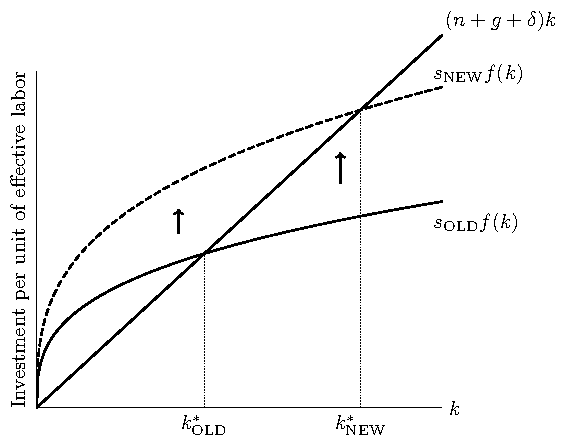
\includegraphics[width=0.75\textwidth]{sections/growth/images/solow_investment_shift}
  \caption{The effect of an increase in the savings rate on investment and steady-state capital}
  \label{fig:solow-investment-shift}
\end{center}
\end{figure}

Using ~\ref{eq:solow-steady-state-k}, the steady-state level of output per worker is
\begin{equation}
y^{*}=\left(k^{*}\right)^{\alpha}=\left(\frac{s}{\delta+n}\right)^{\frac{\alpha}{1-\alpha}}
\label{eq:solow-steady-state-y}
\end{equation}

\subsection{Golden rule of capital accumulation}
What is the impact of a permanent increase in the saving rate $s$ on the steady-state level of consumption per worker $c^{*}$? We start from
\begin{equation}
  c^{*}=(1-s) f\left(k^{*}\right)=f\left(k^{*}\right)-(n+\delta) k^{*}. \label{eq:solow-steady-state-c}
\end{equation}
We know from \eqref{eq:solow-steady-state-k} that $k^{*}$ increases with $s$, but in the expression \eqref{eq:solow-steady-state-c} there is both a positive and a negative effect of $k^{*}$ on $c^{*}$.
When we take the partial derivative, we get
\begin{equation}
  \frac{\partial c^{*}}{\partial s}=\left[f^{\prime}\left(k^{*}\right)-(n+\delta)\right] \frac{\partial k^{*}}{\partial s} \label{eq:solow-c-derivative}
\end{equation}
The sign of this expression will be determined by the sign of the term in square brackets (know that $\frac{\partial k^{*}}{\partial s}>0$ always holds).
Since $f^{\prime}\left(k^{*}\right)$ is very large at small levels of $k^{*}$ (see Figure~\ref{fig:solow-neoclassical-growth}), we can infer that $\frac{\partial c^{*}}{\partial s}>0$ when $k^{*}$ is small, whereas at greater levels of $k^{*}$ it will be the case that $\frac{\partial c^{*}}{\partial s}<0$.
Hence, there is a level of $k^{*}$, referred to as $k^{*, \text{gold}}$, when $\frac{\partial c^{*}}{\partial s}=0$:
\begin{equation}
  \frac{\partial c^{*}}{\partial s}=0 \quad \text { when } f^{\prime}\left(k^{*, \text{gold}}\right)=n+\delta
  \label{eq:solow-golden-rule}
\end{equation}
Beyond this level of $k^{*}$, a further capital accumulation will decrease intensive consumption $c^{*}$.
The savings rate that achieves $k^{*, \text{gold}}$ is referred to as $s^{\text{gold}}$.

\subsection{Convergence}
The Solow-Swan model has strong predictions about convergence, i.e., that countries that start off with a lower level of $k(t)$ should experience a higher growth rate of output per worker.
One way to illustrate this convergence property is as follows.

We keep using the Cobb-Douglas production function $f(k(t))=k(t)^{\alpha}$ and write the growth rate of output per worker as:
\begin{equation}
  \frac{\dot{y}(t)}{y(t)}=\alpha\left(s k(t)^{\alpha-1}-\delta-n\right)
  \label{eq:solow-convergence-growth}
\end{equation}

Since $\frac{Y(t)}{L(t)}=k(t)^{\alpha}=y(t)$, we can express $k(t)$ as $k(t)=y(t)^{\frac{1}{\alpha}}$.
Inserting into the growth equation yields
\begin{equation}
  \frac{\dot{y}(t)}{y(t)}=\alpha\left(s y(t)^{\frac{\alpha-1}{\alpha}}-\delta-n\right)=\alpha\left(\frac{s}{y(t)^{\frac{1-\alpha}{\alpha}}}-\delta-n\right)
  \label{eq:solow-convergence-y}
\end{equation}

Variants of this expression form the basis of the cross-country empirical studies on the determinants of economic growth.
The key prediction concerning convergence is that the growth rate of output per worker should decrease with its initial level, $y(t)$.
In other words, holding all other factors constant, poorer countries should grow faster than richer ones.
A country's growth rate during the convergence process should further increase with its savings rate $s$, and decrease with the population growth rate $n$ and the capital depreciation rate $\delta$.
The growth rate of rich countries that have reached their steady state will depend on the exogenous technological progress parameter.

The convergence result suggests that the poorest countries in the world should experience the highest growth rates.
Although we know that many previously poor countries have experienced very fast growth rates in recent decades---think China, India, Botswana---other countries have experienced stagnant growth or even growth collapses.
Some countries, such as the Democratic Republic of Congo and Zambia, have even seen their levels of income per capita fall by around half from their peak.

\subsection{Extensions}
The simple version of the Solow growth function presented in this document provides the basic intuition behind the important convergence property and the central role played by physical capital accumulation.
It abstracts, however, from numerous factors that are believed to be central for economic growth to occur even in the medium run.
Two of the most important of these factors are technological progress and human capital accumulation.

\subsection{Technological progress}
Technological progress can be readily included in the Solow-Swan model.
Denote the level of technological knowledge at time $t$ as $A(t)$.
Most growth models further assume that technology is primarily labor augmenting, i.e. that $A(t)$ increases workers' level of productivity.
We will refer to the composite production factor $A(t) L(t)$ as effective labor.
The aggregate production function then becomes
\begin{equation}
  Y(t)=F(K(t), A(t) L(t))=K(t)^{\alpha}(A(t) L(t))^{1-\alpha}
  \label{eq:solow-production-tech}
\end{equation}
Let us further assume that the growth rate of technology is exogenously given by
\begin{equation}
  \frac{\dot{A}(t)}{A(t)}=g>0
  \label{eq:solow-tech-growth}
\end{equation}
The intensive form is now written as $\kappa(t)=K(t) / (A(t) L(t))$ and is referred to as capital per unit of effective labor.
The time derivative of $\kappa(t)$ is
\begin{equation}
\begin{aligned}
\dot{\kappa}(t) & =\frac{\dot{K}(t)}{A(t) L(t)}-\frac{K(t) L(t)}{(A(t) L(t))^{2}} \dot{A}(t)-\frac{K(t) A(t)}{(A(t) L(t))^{2}} \dot{L}(t) \\
& =\frac{s Y(t)-\delta K(t)}{A(t) L(t)}-\kappa(t) \frac{\dot{A}(t)}{A(t)}-\kappa(t) \frac{\dot{L}(t)}{L(t)}=s \hat{f}(\kappa(t))-\kappa(t)(\delta+g+n)
\end{aligned}
\label{eq:solow-kappa-dot}
\end{equation}
where $\hat{f}(\kappa(t))=F(K(t), A(t) L(t)) / (A(t) L(t))$.
Similar to our earlier analysis, the economy will be in a steady-state equilibrium when $\dot{\kappa}(t)=0$, which happens at a level $\kappa^{*}=\left(\frac{s}{\delta+g+n}\right)^{\frac{1}{1-\alpha}}$.
The equilibrium level of capital per unit of effective labor thus decreases with the technological growth rate.

Since output per capita can now be expressed as $Y(t) / L(t)=K(t)^{\alpha}(A(t) L(t))^{1-\alpha} / L(t)=A(t) \kappa(t)^{\alpha}$, its growth rate is given by
\begin{equation}
  \frac{\dot{y}(t)}{y(t)}=\frac{\dot{A}(t)}{A(t)}+\alpha \frac{\dot{\kappa}(t)}{\kappa(t)}=g+\alpha\left(\frac{s \hat{f}(\kappa(t))}{\kappa(t)}-\delta-g-n\right)
  \label{eq:solow-output-growth-tech}
\end{equation}
Note that when $\kappa(t)=\kappa^{*}$, the term inside the parentheses will be equal to zero.
The equilibrium growth rate of output per capita is then simply $g>0$.
Hence, rich countries at their equilibrium growth rates will only grow through technological progress.
In the Solow model, this growth rate is exogenously given and we cannot say anything very interesting about it.
Endogenous growth theory extends this framework to derive this growth rate as the result of intentional human investments in research and development (R\&D).

% \subsection{Technological progress}
% Technical change can be embodied or disembodied (see Burmeister and Dobell, 1970, ch. 3). Embodied technical change is only relevant to newly acquired and installed equipment or workers and$ therefore $does not affect the productivity of existing production factors. Disembodied technical progress takes place if, independent of

% \begin{figure}[h]
% \begin{center}
% \begin{tikzpicture}[scale=1.2]
%   % Axes
%   \draw[thick,->] (0,0) -- (7,0) node[right] {$k$};
%   \draw[thick,->] (0,0) -- (0,5) node[above] {$y, sy, (\delta+n)k$};
  
%   % Production function
%   \draw[thick,blue,domain=0:6.5,smooth,variable=\x,samples=100] 
%     plot ({\x},{3*\x^0.4}) node[right] {$f(k)$};
  
%   % Savings function
%   \draw[thick,red,domain=0:6.5,smooth,variable=\x,samples=100] 
%     plot ({\x},{0.8*3*\x^0.4}) node[right] {$sf(k)$};
  
%   % Depreciation line
%   \draw[thick,green!60!black] (0,0) -- (6.5,2.6) node[right] {$(\delta+n)k$};
  
%   % Steady state
%   \draw[dashed] (3.2,0) node[below] {$k^*$} -- (3.2,1.92);
%   \draw[dashed] (0,1.92) node[left] {$y^*$} -- (3.2,1.92);
%   \filldraw (3.2,1.92) circle (2pt);
  
%   % Golden rule point
%   \draw[dashed] (4.5,0) node[below] {$k^{GR}$} -- (4.5,3.6);
%   \filldraw (4.5,1.8) circle (2pt) node[above left] {A};
  
%   % Arrows showing dynamics
%   \draw[->,thick] (1.5,0.2) -- (2.2,0.2);
%   \draw[->,thick] (5,0.2) -- (4.3,0.2);
  
%   % Labels
%   \node at (1.5,-0.5) {$\dot{k}>0$};
%   \node at (5,-0.5) {$\dot{k}<0$};
% \end{tikzpicture}
% \caption{The Solow-Swan model}
% \label{fig:solow-swan-model}
% \end{center}
% \end{figure}

% changes in the production factors, isoquants of the production function shift inwards as time progresses (Burmeister and Dobell, 1970, p. 66). Reasons for this inward shift may be improvements in techniques or organization which increase the productivity of new and old factors alike. Throughout this and the next two chapters we will restrict attention to cases of disembodied technical progress.

% We can represent different cases of factor-augmenting disembodied technical change by writing the production function \eqref{eq:solow-production-function} in the following form:

% \begin{equation}
% Y(t)=F\left(Z_{K}(t) K(t), Z_{L}(t) L(t)\right),
% \label{eq:solow-12-11}
% \end{equation}
%  where $Z_{K}(t)$ and $Z_{L}(t)$ only depend on time, and $Z_{K}(t) K(t)$ and $Z_{L}(t) L(t)$ are ``effective capital'' and ``effective labor'' respectively. Technical progress is purely labor augmenting if $\dot{Z}_{K}(t) := 0$ and $\dot{Z}_{L}(t)>0$, purely capital augmenting if $\dot{Z}_{L}(t) := 0$ and $\dot{Z}_{K}(t)>0$, and equally capital and labor augmenting if $\dot{Z}_{K}(t) := \dot{Z}_{L}(t)>0$.

% Three different concepts of neutrality in the process of technical advance exist in the literature (Burmeister and Dobell, 1970, p. 75; Barro and Sala-i-Martin, 1995, p. 33). Technological change is (a) Harrod neutral if the relative input share $F_{K} K /\left(F_{L} L\right)$ is constant over time for a given capital-output ratio, $K / Y$, (b) Hicks neutral if this share is constant over time for a given capital-labor ratio, $K / L$, and (c) Solow neutral if this share is constant over time for a given labor-output ratio, $L / Y$. In terms of equation \eqref{eq:solow-12-11}, the three cases correspond to, respectively, $Z_{K}(t) := 1, Z_{K}(t) := Z_{L}(t)$, and $Z_{L}(t) := 1$.

% Of course, for the Cobb-Douglas production function the three concepts of neutrality are indistinguishable, since (by redefining terms) we can write:

% \begin{equation}
% \begin{aligned}
% & Y(t)=\left[Z_{K}(t) K(t)\right]^{\alpha} L(t)^{1-\alpha} \quad \Leftrightarrow \\
% & Y(t)=K(t)^{\alpha}\left[Z_{L}(t) L(t)\right]^{1-\alpha} \quad \\
% & Y(t)=Z(t) K(t)^{\alpha} L(t)^{1-\alpha} \quad
% \end{aligned} \quad \begin{aligned}
% & \text { for } Z_{L}(t) := Z_{K}(t)^{\alpha /(1-\alpha)} \\
% & Y(t)=Z_{K}(t)^{\alpha}.
% \end{aligned}
% \label{eq:solow-12-12}
% \end{equation}

% For non-Cobb-Douglas cases, however, the different neutrality concepts have different implications for balanced growth. Barro and Sala-i-Martin (1995, pp. 54-55) show, for example, that technical progress must be Harrod neutral (labor augmenting) for the model to have a steady state with a constant growth rate. In a steady state
% we must have a constant capital-output ratio and it can be shown that for forms of technological progress that are not Harrod neutral, one of the factor shares approaches zero if the capital-output ratio is to be constant. So if we wish to have balanced growth and be able to consider a non-unitary substitution elasticity between capital and labor, we must assume Harrod-neutral technical progress. The remainder of the discussion in this section will thus assume that Harrod neutrality holds.

% The production function is written as:

% \begin{equation}
% Y(t)=F(K(t), N(t)),
% \label{eq:solow-12-13}
% \end{equation}
%  where $N(t)$ measures the effective amount of labor $(N(t) := Z(t) L(t))$ and we assume that technical progress occurs at a constant exponential rate:

% \begin{equation}
% \frac{\dot{Z}(t)}{Z(t)}=n_{Z}, \quad Z(t)=Z(0) e^{n_{Z} t}.
% \label{eq:solow-12-14}
% \end{equation}

% Since the labor force itself grows exponentially at a constant rate $n$ (see \eqref{eq:solow-capital-accumulation}), the effective labor force grows at a constant exponential rate $n+n_{Z}$, i.e.:

% \begin{equation}
% \frac{\dot{N}(t)}{N(t)} := \frac{\dot{Z}(t)}{Z(t)}+\frac{\dot{L}(t)}{L(t)}=n_{Z}+n.
% \label{eq:solow-12-15}
% \end{equation}

% By measuring output and capital per unit of effective labor, i.e. $y(t) := Y(t) / N(t)$ and $k(t) := K(t) / N(t)$, and following the standard solution procedure explained above (in Intermezzo 12.1), the fundamental differential equation for $k(t)$ is obtained:

% \begin{equation}
% \dot{k}(t)=s f(k(t))-\left(\delta+n+n_{Z}\right) k(t).
% \label{eq:solow-12-16}
% \end{equation}

% In the steady state, $k^{*}=s y^{*} /\left(\delta+n+n_{Z}\right)$, so that output and the capital stock grow at the same rate as the effective labor input. Hence, equation \eqref{eq:solow-12-10} is changed to:

% \begin{equation}
% \left(\frac{\dot{Y}(t)}{Y(t)}\right)^{*}=\left(\frac{\dot{K}(t)}{K(t)}\right)^{*}=\left(\frac{\dot{I}(t)}{I(t)}\right)^{*}=\left(\frac{\dot{S}(t)}{S(t)}\right)^{*}=\frac{\dot{N}(t)}{N(t)}=\frac{\dot{L}(t)}{L(t)}+\frac{\dot{Z}(t)}{Z(t)}=n+n_{Z}.
% \label{eq:solow-12-17}
% \end{equation}

% Hence, exactly the same qualitative conclusions are obtained as in the model without technological advance. Long-term balanced growth merely depends on the exogenous factors $n$ and $n_{Z}$. Note that stylized fact (SF1) is accounted for as output per worker grows at an exponential rate $n_{Z}$ along the balanced growth path.

% \subsection{Properties of the Solow-Swan model}
% In this section we study the most important properties of the Solow-Swan model. In particular, we look at (a) the golden rule and the issue of over-saving, (b) the transitional dynamics implied by the model as well as the concept of absolute versus conditional convergence, and (c) the speed of dynamic adjustment.

% \subsection{The golden rule of capital accumulation}
% One of the implications of the model developed thus far is that, even though longterm balanced growth is exogenous (and equal to $n := n+n_{Z}$ ), the levels of output,
% capital, and consumption are critically affected by the level of the savings rate. In other words, even though $s$ does not affect long-term growth it does affect the path along which the economy grows. This prompts the issue concerning the relative welfare ranking for these different paths. To the extent that the policy maker can affect $s$, he can also select the path on which the economy finds itself. We first consider steady-state paths and, to keep things simple, we assume that there is no technical progress (i.e. $n_{Z}=0$ and $n=n$ ).

% In the steady state, equation \eqref{eq:solow-fundamental-equation} implies $a unique implicit relationship between the savings rate and the equilibrium capital-labor ratio which can be written as $s f\left(k^{*}\right)=(\delta+n) k^{*}$. By using the implicit function theorem we thus find that $k^{*}$ depends on $s$ :

% \begin{equation}
% k^{*}=k^{*}(s),
% \label{eq:solow-12-18}
% \end{equation}

% with $d k^{*} / d s=y^{*} /\left[\delta+n-s f^{\prime}\left(k^{*}\right)\right]>0$. Suppose that the policy maker is interested in steady-state per capita consumption which can be written as a function of the savings rate:

% \begin{equation}
% c^{*}(s)=(1-s) f\left(k^{*}(s)\right)=f\left(k^{*}(s)\right)-(\delta+n) k^{*}(s).
% \label{eq:solow-12-19}
% \end{equation}

% In terms of Figure~\ref{fig:solow-swan-model}, $c^{*}(s)$ represents the vertical distance between the production function and the required-replacement line in the steady state. In Figure~\ref{fig:solow-per-capita-consumption} we plot $c^{*}(s)$ for different savings rates. Any output not needed to replace the existing capital stock per worker in the steady state can be consumed. Per capita consumption is at its maximum if the savings rate satisfies $d c^{*}(s) / d s=0$, or:

% \begin{equation}
% \frac{d c^{*}(s)}{d s}=\left[f^{\prime}\left(k^{*}(s)\right)-(\delta+n)\right] \cdot \frac{d k^{*}(s)}{d s}=0.
% \label{eq:solow-12-20}
% \end{equation}

% In terms of Figure~\ref{fig:solow-swan-model}, per capita consumption is at its maximum at point A$ where $the slope of the production function equals the slope of the required-replacement function. In view of \eqref{eq:solow-12-20}, the golden rule savings rate, $s^{G R}$, satisfies:

% \begin{equation}
% f^{\prime}\left(k^{*}\left(s^{G R}\right)\right)=\delta+n.
% \label{eq:solow-12-21}
% \end{equation}

% The golden rule savings rate is associated with point $\mathrm{E}_{1}$ in Figure~\ref{fig:solow-per-capita-consumption}. Burmeister and Dobell (1970, pp. 52-53) provide the economic intuition behind the result in \eqref{eq:solow-12-21}. The produced asset (the physical capital stock) yields an own-rate of return equal to $f^{\prime}-\delta$, whereas the non-produced primary good (labor) can be interpreted as yielding an own-rate of return $n=n$. Intuitively, the efficient outcome occurs if the rates of return on the two assets are equalized, i.e. if the equality in \eqref{eq:solow-12-21} holds.

% Since $s^{G R} f\left(k^{*}\left(s^{G R}\right)\right)=(\delta+n) k^{*}\left(s^{G R}\right)$ we can rewrite the expression in \eqref{eq:solow-12-21} as:

% \begin{equation}
% s^{G R}=\frac{k^{*}\left(s^{G R}\right) \cdot f^{\prime}\left(k^{*}\left(s^{G R}\right)\right)}{f\left(k^{*}\left(s^{G R}\right)\right)}.
% \label{eq:solow-12-22}
% \end{equation}

% Equation \eqref{eq:solow-12-22} shows that the golden rule savings rate is equal to the share of capital income in national income (which itself in general depends on the golden rule savings rate). In the Cobb-Douglas case, with $f(\cdot)=k(t)^{\alpha}, \alpha$ represents the capital income share so that the golden rule savings rate equals $s^{G R}=\alpha$.

% We are now in a position to discuss the concept of dynamic inefficiency. We call an economy dynamically inefficient if it is possible to make everybody at least as well

% \begin{figure}[h]
% \begin{center}
%   % \includegraphics[width=\textwidth]{2025_09_07_2ad0768dad3918af3d98g-09} % Missing image file
% \caption{Per capita consumption and the savings rate}
% \label{fig:solow-per-capita-consumption}
% \end{center}
% \end{figure}

% off (and some strictly better off) by reducing the capital stock. Consider the situation in Figure~\ref{fig:solow-per-capita-consumption}, and assume that the actual steady-state savings rate is $s_{0}$ so that the economy is at point $\mathrm{E}_{0}$. Since this savings rate exceeds the golden rule savings rate ( $s_{0}>s^{G R}$ ), per capita consumption is lower than under the golden rule. It is not difficult to show that point $E_{0}$ is dynamically inefficient in the sense that higher per capita consumption can be attained by reducing the savings rate. Figure~\ref{fig:solow-per-capita-consumption} shows that a reduction in the savings rate from $s_{0}$ to $s^{G R}$ would move the steady state from $\mathrm{E}_{0}$ to $\mathrm{E}_{1}$ and lead to higher per capita steady-state consumption. With the aid of Figure~\ref{fig:solow-golden-rule-transition} we can figure out what happens to per capita consumption during the transitional phase. The economy is initially at point $\mathrm{E}_{0}$ and the initial steady-state capital-labor ratio is $k_{0}^{*}$. A reduction in the savings rate (from $s_{0}$ to $s^{G R}$ ) rotates the per capita consumption schedule in a counter-clockwise fashion and the economy jumps from $\mathrm{E}_{0}$ to A at impact. Since the transition towards the golden-rule capital-labor ratio $k^{G R}$ is stable, the economy moves from A to the new steady-state point $\mathrm{E}_{1}$ as $k(t)$ falls towards $k^{G R}$ during transition. Hence, as a result of the decrease in the savings rate, consumption is higher than it would have been, both during transition and in the new steady state. It follows that the reduction in $s$ is Pareto improving, and we can conclude that savings rates exceeding $s^{G R}$ are dynamically inefficient.

% The same conclusion does not hold if the savings rate falls short of $s^{G R}$ as the Pareto-optimality property cannot be demonstrated unambiguously. Consider an economy in which the savings rate falls short of its golden rule level, i.e. $s_{1}<s^{G R}$. In terms of Figures~\ref{fig:solow-per-capita-consumption} and \ref{fig:solow-golden-rule-transition}, the economy is initially at point $\mathrm{E}_{2}$. An increase in the savings rate from $s_{1}$ to $s^{G R}$ still leads to an increase in steady-state per capita consumption. During transition, however, per capita consumption will have to fall before it can settle at its higher steady-state level prescribed by the golden rule. In terms of Figure~\ref{fig:solow-golden-rule-transition}, at impact the economy jumps from $E_{2}$ to $B$ as the savings rate is increased. During part of the transition, consumption is lower than it would have been in the absence of the shock. Since we have no welfare function to evaluate the uneven path of per capita consumption, we cannot determine whether the increase in $s$ is Pareto improving in this case.

% \begin{figure}[h]
% \begin{center}
%   % \includegraphics[width=\textwidth]{2025_09_07_2ad0768dad3918af3d98g-10} % Missing image file
% \caption{Per capita consumption during transition to its golden rule level}
% \label{fig:solow-golden-rule-transition}
% \end{center}
% \end{figure}

% \subsection{Transitional dynamics and convergence}
% Up to now attention has been focused on steady-state issues. We now return to the model with exogenous technical change, the fundamental equation of which is given in \eqref{eq:solow-12-16}. By defining the growth rate of $k(t)$ as $\gamma_{k}(t) := \dot{k}(t) / k(t)$, we derive from \eqref{eq:solow-12-16}:

% \begin{equation}
% \gamma_{k}(t) := s \cdot \frac{f(k(t))}{k(t)}-(\delta+n),
% \label{eq:solow-12-23}
% \end{equation}
%  where $n := n+n_{Z}$. In Figure~\ref{fig:solow-growth-convergence} this growth rate is represented by the vertical difference between the two lines. ${ }^{5}$ An immediate implication of \eqref{eq:solow-12-23}, or Figure~\ref{fig:solow-growth-convergence} for that matter, is that countries with little capital and low output (in efficiency units) grow faster than countries with a lot of capital and high output. The further away a country is from the steady state, the higher will be its growth rate. In other words, poor and rich countries should converge!

% This suggests that there is a simple empirical test of the Solow-Swan model which is based on the convergence property of output in a cross-section of different countries. We take a group of closed economies (since the Solow-Swan model refers to the closed economy) and assume that they are similar in the sense that they possess the same structural parameters, $s, n$, and $\delta$, and the same production function, so that in theory they have the same steady state. The so-called absolute convergence hypothesis (ACH) then suggests that poor countries should grow faster than rich countries. Barro and Sala-i-Martin (1995, p. 27), using a sample of 118 countries, regress the growth rate in per capita GDP during the period 1960-1985 on the logarithm of per capita GDP in the base year 1960. The results of their regression are dismal: instead of finding a negative effect as predicted by the ACH , they find a slight positive effect, i.e. countries that were rich in the base year ended up growing faster than poor countries did. Absolute convergence does not seem to hold and (Paul Romer's) stylized fact (SF7) is verified by the data.

% \footnote{The Inada conditions ensure that $\lim _{k \rightarrow 0} s f(k) / k=\infty$ (vertical at the origin) and $\lim _{k \rightarrow \infty} s f(k) / k=0$ (approaches horizontal axis asymptotically).
% }\begin{figure}[h]
% \begin{center}
%   % \includegraphics[width=\textwidth]{2025_09_07_2ad0768dad3918af3d98g-11} % Missing image file
% \caption{Growth convergence}
% \label{fig:solow-growth-convergence}
% \end{center}
% \end{figure}

% This rejection of the ACH does not necessarily mean that the Solow-Swan model is refuted because one of the identifying assumptions underlying the regression results could be false. For example, if a rich country has a higher savings rate than a poor country, it could actually be further from its (higher) steady state than the poor country is from its steady state. The Solow-Swan model then predicts that the rich country will be growing faster than the poor country, as indeed the empirical results of Barro and Sala-i-Martin (1995) suggest. We demonstrate this result in Figure~\ref{fig:solow-conditional-convergence} where $s_{P}$ and $s_{R}$ are the savings rates of the poor and the rich country, respectively, and $\left(k^{*}\right)^{P}$ and $\left(k^{*}\right)^{R}$ are the corresponding steady states. If the poor country is initially at $k^{P}(0)$ and the rich country at $k^{R}(0)$, the former will grow slower than the latter (the vertical distance CD is larger than AB ).

% A refined test of the Solow-Swan model makes use of the conditional convergence hypothesis (CCH) according to which truly similar countries should converge. Barro and Sala-i-Martin (1995, pp. 27-28) show that convergence does appear to take place for the twenty original OECD countries and a fortiori for the different states in the US. This suggests that the CCH is not grossly at odds with the data, which is good news for the Solow-Swan model (and bad news for some of the endogenous growth models discussed in Chapter 14 below).

% \subsection{The speed of adjustment}
% The convergence property is not the only testable implication of the Solow-Swan model. Apart from testing whether economies converge, another issue concerns how fast they converge. In order to study this issue further we follow Burmeister and Dobell (1970, pp. 53-56) and Barro and Sala-i-Martin (1995, pp. 37-39, 53) by focusing on the Cobb-Douglas case for which $f(\cdot)=k(t)^{\alpha}$, and the fundamental differential equation \eqref{eq:solow-12-16} becomes:

% \begin{equation}
% \dot{k}(t)=s k(t)^{\alpha}-(\delta+n) k(t).
% \label{eq:solow-12-24}
% \end{equation}

% \begin{figure}[h]
% \begin{center}
%   % \includegraphics[width=\textwidth]{2025_09_07_2ad0768dad3918af3d98g-12} % Missing image file
% \caption{Conditional growth convergence}
% \label{fig:solow-conditional-convergence}
% \end{center}
% \end{figure}

% An exact analytical solution to this differential equation is not available because $k(t)$ enters non-linearly on the right-hand side of \eqref{eq:solow-12-24} (as $0<\alpha<1$ ). By using a firstorder Taylor approximation around the steady-state capital intensity, $k^{*}$, we obtain:

% \begin{equation}
% \begin{aligned}
% s k(t)^{\alpha} & \approx s\left(k^{*}\right)^{\alpha}+s \alpha\left(k^{*}\right)^{\alpha-1}\left[k(t)-k^{*}\right] \\
% & =(\delta+n) k^{*}+\alpha(\delta+n)\left[k(t)-k^{*}\right]
% \end{aligned}
% \label{eq:solow-12-25}
% \end{equation}
% where we have used the fact that $s\left(k^{*}\right)^{\alpha}=(\delta+n) k^{*}$ in getting from the first to the second expression. Using \eqref{eq:solow-12-25} in \eqref{eq:solow-12-24} we obtain the linearized differential equation for $k(t)$:

% \begin{equation}
% \dot{k}(t)=-\beta\left[k(t)-k^{*}\right], \quad \beta :=(1-\alpha)(\delta+n)>0
% \label{eq:solow-12-26}
% \end{equation}

% Denoting the capital intensity in the base period by $k(0)$, the solution to \eqref{eq:solow-12-26} can be obtained by standard methods:

% \begin{equation}
% k(t)=k^{*}+\left[k(0)-k^{*}\right] e^{-\beta t}
% \label{eq:solow-12-27}
% \end{equation}
%  where $k^{*}$ is the steady-state capital intensity to which the economy converges in the long run, and where $\beta$ measures the speed of convergence.

% It is not difficult to deduce the speed of adjustment in the growth rate of output for the Cobb-Douglas case. ${ }^{6}$ Indeed, dividing both sides of \eqref{eq:solow-12-26} by $k(t)$, noting that $\dot{k}(t) / k(t)=d \log k(t) / d t, d \log y(t) / d t=\alpha d \log k(t) / d t$, and using the approximation $\log \left(k(t) / k^{*}\right)=1-k^{*} / k(t)$, we find:

% \begin{equation}
% \frac{d \log y(t)}{d t}=-\beta\left[\log y(t)-\log y^{*}\right]
% \label{eq:solow-12-28}
% \end{equation}

% \footnote{The more general case is covered by Barro and Sala-i-Martin (1995, p. 24).
% }
% which$ implies $that:
% \begin{equation}
% \log y(t)=\log y^{*}+\left[\log y(0)-\log y^{*}\right] e^{-\beta t}.
% \label{eq:solow-12-29}
% \end{equation}

% Hence, $\beta$ is the common (approximate) adjustment speed for $k(t), \log k(t), y(t)$, and $\log y(t)$ toward their respective steady-states.

% The intuitive interpretation of $\beta$ is as follows: $\zeta \times 100 \%$ of the gap between $k(t)$ and $k^{*}$ is eliminated after a time interval of $t_{\zeta}$ :

% \begin{equation}
% t_{\zeta} :=-\frac{\log (1-\zeta)}{\beta}.
% \label{eq:solow-12-30}
% \end{equation}

% Hence, the half-life of the adjustment $\left(\zeta=\frac{1}{2}\right)$ equals $t_{1 / 2}=\log 2 / \beta=0.693 / \beta .^{7}$ Some back-of-the-envelope computations based on representative values of $n=0.01$ (per annum), $n_{\mathrm{Z}}=0.02, \delta=0.05$, and $\alpha=1 / 3$ yield the value of $\beta=0.0533$ (5.33\% per annum) and an estimated half-life of $t_{1 / 2}=13$ years. Transition is thus relatively fast, at least from a growth perspective. ${ }^{8}$ As Barro and Sala-i-Martin (1995, p. 38) indicate, however, this estimate is far too high to accord with empirical evidence. They suggest that $\beta$ is more likely to be in the range of $2 \%$ per annum (instead of $5.33 \%$ ). So here is a real problem confronting the Solow-Swan model. In order for it to generate a realistic convergence rate of $2 \%$, for given values of $\delta$ and $n$, the capital share must be unrealistically high (a value of $\alpha=\frac{3}{4}$ actually yields an estimate of $\beta=0.02$ )! One way to get the Solow-Swan model in line with reality is to assume a broad measure of capital to include human as well as physical capital. This is indeed the approach taken by Mankiw, Romer, and Weil (1992).

% \subsection{Human capital to the rescue}
% Mankiw, Romer, and Weil (1992, p. 415) start their analysis by using real world data to estimate the textbook Solow model. They show that, though the model appears to fit the data quite well, some of the parameter estimates are not entirely satisfactory. For example, the estimated capital coefficient is much larger than the actual capital share of about one third. So either their Cobb-Douglas technology assumption is inappropriate or there is a serious mis-measurement of the capital input. They adopt the latter stance and suggest that the convergence conundrum of the Solow-Swan model disappears if the production function is modified to include human capital:

% \begin{equation}
% Y(t)=K(t)^{\alpha_{K}} H(t)^{\alpha_{H}}[Z(t) L(t)]^{1-\alpha_{K}-\alpha_{H}},
% \label{eq:solow-12-31}
% \end{equation}
%  where $H(t)$ is the stock of human capital and $\alpha_{K}$ and $\alpha_{H}$ are the efficiency parameters of the two types of capital ( $0<\alpha_{K}, \alpha_{H}, \alpha_{K}+\alpha_{H}<1$ ). In close accordance with the Solow-Swan model, productivity and population growth are both exponential $\left(\dot{Z}(t) / Z(t)=n_{Z}\right.$ and $\dot{L}(t) / L(t)=n$ ) and the accumulation equations for the two types of capital and the production function can be written in effective labor units as:

% \begin{equation}
% \dot{k}(t)=s_{K} y(t)-\left(\delta_{K}+n\right) k(t),
% \label{eq:solow-12-32}
% \end{equation}

% \footnote{See also Chapter 7$ where $we compute the convergence speed of the unemployment rate in a discretetime setting.
% ${ }^{8}$ Note that \textcite{sato1963fiscal} actually complains about the startlingly low transition speed implied by the Solow-Swan model. His object of study is fiscal policy and business cycle phenomena. In this context convergence of $5 \%$ per annum is slow.$ hence $the different conclusion.
% }
% \begin{equation}
% \begin{aligned}
% & \dot{h}(t)=s_{H} y(t)-\left(\delta_{H}+n\right) h(t) \\
% & y(t)=k(t)^{\alpha_{K}} h(t)^{\alpha_{H}}
% \end{aligned}
% \label{eq:solow-12-33-34}
% \end{equation}
% where $k(t) := K(t) /[Z(t) L(t)]$, $h(t) := H(t) /[Z(t) L(t)]$, $y(t) := Y(t) /[Z(t) L(t)]$, $n := n_{Z}+n$, and $s_{K}$ and $s_{H}$ represent the propensities to accumulate physical and human capital, respectively. The depreciation rates of physical and human capital are denoted by, respectively, $\delta_{K}$ and $\delta_{H}$. ${ }^{9}$ The production functions of the two types of capital are assumed to be equal.

% \subsection{Stability}
% In order to study the stability properties of the model, we must first derive its phase diagram. The $\dot{k}(t)=0$ line is obtained by substituting (12.34) into \eqref{eq:solow-12-32} and rearranging terms somewhat:

% \begin{equation}
% h(t)=\left(\frac{\delta_{K}+n}{s_{K}}\right)^{1 / \alpha_{H}} \cdot k(t)^{\left(1-\alpha_{K}\right) / \alpha_{H}},
% \label{eq:solow-12-35}
% \end{equation}
% where we note that the exponent for $k(t)$ exceeds unity $\left(\left(1-\alpha_{K}\right) / \alpha_{H}>1\right)$. In terms of Figure~\ref{fig:solow-augmented-solow-swan}, the $\dot{k}(t)=0$ line passes through the origin and is convex. For points to the right (left) of the line, the physical capital stock falls (rises) over time. This has been indicated with horizontal arrows in Figure~\ref{fig:solow-augmented-solow-swan}. In a similar fashion, the $\dot{h}(t)=0$ line is obtain by using (12.34) in \eqref{eq:solow-12-33-34}:

% \begin{equation}
% h(t)=\left(\frac{s_{H}}{\delta_{H}+n}\right)^{1 /\left(1-\alpha_{H}\right)} \cdot k(t)^{\alpha_{K} /\left(1-\alpha_{H}\right)}
% \label{eq:solow-12-36}
% \end{equation}
% where we observe that the exponent for $k(t)$ falls short of unity $\left(\alpha_{K} /\left(1-\alpha_{H}\right)<1\right)$. The $\dot{h}(t)=0$ line passes through the origin and is concave. For points above (below) the line, the human capital stock falls (rises) over time-see the vertical arrows in Figure~\ref{fig:solow-augmented-solow-swan}. Since there are decreasing returns to the two types of capital in combination ( $\alpha_{K}+\alpha_{H}<1$ ) the model possesses a unique steady state for which $\dot{k}(t)=\dot{h}(t)=0$, $k(t)=k^{*}$, and $h(t)=h^{*}$. By using \eqref{eq:solow-12-35}-\eqref{eq:solow-12-36} we obtain:

% \begin{equation}
% \begin{aligned}
% & k^{*}=\left(\left(\frac{s_{K}}{\delta_{K}+n}\right)^{1-\alpha_{H}}\left(\frac{s_{H}}{\delta_{H}+n}\right)^{\alpha_{H}}\right)^{1 /\left(1-\alpha_{K}-\alpha_{H}\right)} \\
% & h^{*}=\left(\left(\frac{s_{K}}{\delta_{K}+n}\right)^{\alpha_{K}}\left(\frac{s_{H}}{\delta_{H}+n}\right)^{1-\alpha_{K}}\right)^{1 /\left(1-\alpha_{K}-\alpha_{H}\right)}
% \end{aligned}
% \label{eq:solow-12-37}
% \end{equation}

% The configuration of arrows in Figure~\ref{fig:solow-augmented-solow-swan} confirms that the model is stable. Along the balanced growth path, $Y(t), K(t), H(t)$, and $C(t)$ all grow at the same exponential growth rate, $n$, just as in the standard Solow-Swan model discussed above.

% \subsection{Empirical performance}
% By substituting $k^{*}$ and $h^{*}$ into the (logarithm of the) production function (12.34)$ we obtain $an estimable expression for per capita output along the balanced growth path:

% \begin{equation}
% \log \left(\frac{Y(t)}{L(t)}\right)^{*}=\log Z(0)+n_{Z} t-\frac{\alpha_{K} \log \left(\delta_{K}+n_{Z}+n\right)+\alpha_{H} \log \left(\delta_{H}+n_{Z}+n\right)}{1-\alpha_{K}-\alpha_{H}}
% \label{eq:solow-12-38}
% \end{equation}

% \footnote{We use a slightly more general version of the Mankiw-Romer-Weil model by allowing $\delta_{K}$ to differ from $\delta_{H}$. This model was also studied by Solow (1999, pp. 653-655).
% }\begin{figure}[h]
% \begin{center}
%   % \includegraphics[width=\textwidth]{2025_09_07_2ad0768dad3918af3d98g-15} % Missing image file
% \caption{Augmented Solow-Swan model}
% \label{fig:solow-augmented-solow-swan}
% \end{center}
% \end{figure}

% \begin{equation}
% +\frac{\alpha_{K}}{1-\alpha_{K}-\alpha_{H}} \log s_{K}+\frac{\alpha_{H}}{1-\alpha_{K}-\alpha_{H}} \log s_{H},
% \label{eq:solow-12-39}
% \end{equation}
% where we recall that $\log y(t) := \log (Y(t) / L(t))-\log Z(t)$ and we have used the second expression in \eqref{eq:solow-12-14} to write $\log Z(t)=\log Z(0)+n_{Z} t$. Mankiw, Romer, and Weil (1992, p. 417) suggest approximate guesses for $\alpha_{K}=\frac{1}{3}$ and $\alpha_{H}$ between $\frac{1}{3}$ and $\frac{4}{9}$. The latter guess is based on the observation that in the US manufacturing sector the minimum wage is between a third and a half of the average wage. By interpreting the minimum wage as the return to labor without any human capital (so-called ``raw'' labor), this means that between half and two thirds of the total payment to labor represents the return to human capital. Since an income share of ( $1-\alpha_{K}$ ) is left after payments to owners of physical capital are taken care of, this implies $\frac{1}{2}\left(1-\alpha_{K}\right)<\alpha_{H}<\frac{2}{3}\left(1-\alpha_{K}\right)$ or $\frac{1}{3}<\alpha_{H}<\frac{4}{9} .{ }^{10}$

% As a result of the inclusion of human capital, the model is much better equipped to explain large cross-country income differences for relatively small differences between, for example, savings rates ( $s_{K}$ and $s_{H}$ ) and population growth rates ( $n$ ). This is apparent from equation \eqref{eq:solow-12-39}. An increase in $s_{K}$, for example, induces higher income in efficiency units just as in the standard Solow-Swan model (see \eqref{eq:solow-12-32}) but also raises the stock of human wealth in efficiency units. By adding human capital to the model, the elasticity of $s_{K}$ in \eqref{eq:solow-12-39} is of the order of unity rather than one half which is predicted by the standard Solow-Swan model. A similar conclusion holds for a change in $n$. An increase in $n$ reduces income because both physical and human capital are spread out over more souls and the elasticity $\partial \log (Y / L)^{*} / \partial n=-\left(\alpha_{K}+\alpha_{H}\right) /\left(1-\alpha_{K}-\alpha_{H}\right)$ is not $-\frac{1}{2}$, as in the Solow-Swan

% \footnote{Ingenious as it is, this approach to estimating the income share of human capital is not without dangers, especially in Europe$ where $the minimum wage is policy manipulated rather than market determined.
% }
% model, but (for $\alpha_{H}=\frac{1}{3}$ ) a staggering -2! See Romer (2012) for a further numerical example.

% Not surprisingly, the inclusion of a human capital variable works pretty well empirically; the estimated coefficient for $\alpha_{H}$ is highly significant and lies between 0.28 and 0.37 (Mankiw, Romer, and Weil, 1992, p. 420). The convergence property of the augmented Solow-Swan model is also much better. Indeed, for the special case with $\delta_{K}=\delta_{H}=\delta$, the convergence speed is given by $\beta :=\left(1-\alpha_{K}-\alpha_{H}\right)(n+ \delta$ ) which can be made in accordance with the observed empirical estimate of $\hat{\beta}=$ 0.02 without too much trouble. Hence, by this very simple and intuitively plausible adjustment the Solow-Swan model can be salvaged from the dustbin of history. The speed of convergence it$ implies $can be made to fit the real world.

% \subsection{Macroeconomic applications of the Solow-Swan model}
% The Solow-Swan model can also be used to study traditional macroeconomic issues such as the effect of fiscal policy and the issue of debt versus tax financing and Ricardian equivalence. In order to keep things simple, we return to the standard SolowSwan model in which there is only physical capital.

% \subsection{Fiscal policy in the Solow model}
% Suppose that the government consumes $G(t)$ units of output so that aggregate demand in the goods market is:

% \begin{equation}
% Y(t)=C(t)+I(t)+G(t) .
% \end{equation}

% Aggregate saving is proportional to after-tax income, so that (12.2) is modified to:

% \begin{equation}
% S(t)=s[Y(t)-T(t)],
% \end{equation}
% where $T(t)$ is the lump-sum tax. Since $S(t) := Y(t)-C(t)-T(t)$ any primary government deficit must be compensated for by an excess of private saving over investment, i.e. $G(t)-T(t)=S(t)-I(t)$. The government budget identity is given by:

% \begin{equation}
% \dot{B}(t)=r(t) B(t)+G(t)-T(t),
% \end{equation}
%  where $B(t)$ is government debt and $r(t)$ is the real interest rate which, under the competitive conditions assumed in the Solow-Swan model, equals the net marginal productivity of capital: ${ }^{11}$

% \begin{equation}
% r(t)=f^{\prime}(k(t))-\delta .
% \end{equation}

% By writing all variables in terms of effective labor units, the model can be condensed to the following two equations:

% \begin{equation}
% \begin{aligned}
% \dot{k}(t) & =f(k(t))-(\delta+n) k(t)-c(t)-g(t) \\
% & =s f(k(t))-(\delta+n) k(t)+(1-s) \tau(t)-g(t), \\
% \dot{b}(t) & =\left[f^{\prime}(k(t))-\delta-n\right] b(t)+g(t)-\tau(t),
% \end{aligned}
% \end{equation}

% \footnote{This result is demonstrated more formally below. See section 13.1.2.
% } where $\tau(t) := T(t) / N(t), g(t) := G(t) / N(t)$, and $b(t) := B(t) / N(t)$. In the remainder of this subsection we assume that (i) government consumption per efficiency unit of labor is time-invariant, i.e. $g(t)=g$, and (ii) the economy is dynamically efficient, i.e. the initial capital stock, $k_{0}^{*}$, falls short of its golden-rule level so that the net interest rate is positive, $r_{0}^{*}-n := f^{\prime}\left(k_{0}^{*}\right)-\delta-n>0$.

% \subsection{Tax-financed increase in government consumption}
% Under pure tax financing and in the absence of initial government $\operatorname{debt}(\dot{b}(t)=b(t)=$ 0 ), the government budget identity reduces to $\tau(t) := g$, i.e. the tax is also timeinvariant. By substituting this expression into (12.44) we obtain:

% \begin{equation}
% \dot{k}(t)=s[f(k(t))-g]-(\delta+n) k(t) .
% \end{equation}

% The economy can be analysed with the aid of (12.46) alone-see Figure~\ref{fig:solow-fiscal-policy}. In the absence of government consumption ( $g=0$ ), the unique (and stable) steady-state equilibrium is at point $\mathrm{E}_{0}$. An increase in government consumption shifts the savings line down which results in multiple equilibria (or even no equilibria). Of these equilibria, the one at point A is unstable and that at $\mathrm{E}_{1}$ is stable. Restricting attention to the stable equilibrium, we find that fiscal policy crowds out the physical capital stock in the long run, from $k_{0}^{*}$ to $k_{1}^{*}$. At impact, the capital stock is predetermined ( $k(0)=k_{0}^{*}$ ), private consumption and net investment (in efficiency units of labor) both fall $(d c(0) / d g=-(1-s)<0$ and $d \dot{k}(0) / d g=-s<0$ ) but output is unchanged $(d y(0) / d g=0)$. Over time, as the capital stock gradually falls towards its new steady-state value, output and private consumption per effective labor unit fall. The long-run effects are given by:

% \begin{equation}
% \begin{aligned}
% & \frac{d y(\infty)}{d g}=\frac{f^{\prime}\left(k_{0}^{*}\right) d k(\infty)}{d g}=-\frac{s f^{\prime}\left(k_{0}^{*}\right)}{\delta+n-s f^{\prime}\left(k_{0}^{*}\right)}<0, \\
% & \frac{d c(\infty)}{d g}=\left(r_{0}^{*}-n\right) \frac{d k(\infty)}{d g}-1<-1,
% \end{aligned}
% \end{equation}
% where the sign in (12.47) follows readily from the fact that the required investment line is steeper than the savings line at the steady-state point $\mathrm{E}_{0}$, i.e. $\delta+n>s f^{\prime}\left(k_{0}^{*}\right)$, as can indeed be seen in Figure~\ref{fig:solow-fiscal-policy}. Private consumption is crowded out more than one-for-one by public consumption in the long run.

% \subsection{Bond-financed tax cut}
% Next we consider the issue of bond financing. If the government increases its consumption without at the same time raising $\tau(t)$ by the same amount, a primary deficit will be opened up which, according to (12.45), will lead to an ever-increasing explosive process for government debt (since $r>n$ by assumption in (12.45)). In order to avoid this economically rather uninteresting result, we postulate a debt stabilization rule, a variation of which was suggested by Buiter (1988, p. 288):

% \begin{equation}
% \tau(t)=\tau_{0}+\xi b(t), \quad \xi>r-n .
% \end{equation}

% \begin{figure}[h]
% \begin{center}
%   % \includegraphics[width=\textwidth]{2025_09_07_2ad0768dad3918af3d98g-18} % Missing image file
% \caption{Fiscal policy in the Solow-Swan model}
% \label{fig:solow-fiscal-policy}
% \end{center}
% \end{figure}

% The tax thus depends positively on the outstanding stock of government debt. By substituting (12.49) into (12.45)$ we obtain $a stable debt process: ${ }^{12}$

% \begin{equation}
% \dot{b}(t)=\left[f^{\prime}(k(t))-\delta-n-\xi\right] b(t)+g-\tau_{0} .
% \end{equation}

% The dynamic properties of the economy can be illustrated with the aid of a phase diagram in ( $b, k$ ) space-see Figure~\ref{fig:solow-ricardian-non-equivalence}. By combining (12.44) and (12.49) and setting $g(t)=g$ we obtain the following expression:

% \begin{equation}
% \dot{k}(t)=s f(k(t))-(\delta+n) k(t)+(1-s)\left[\tau_{0}+\xi b(t)\right]-g .
% \end{equation}

% The slope of the $\dot{k}=0$ line (evaluated at the steady state $\left(k_{0}^{*}, b_{0}^{*}\right)$ ) is obtained from (12.51) in the usual fashion:

% \begin{equation}
% \left(\frac{d b(t)}{d k(t)}\right)_{\dot{k}(t)=0}=\frac{\delta+n-s f^{\prime}\left(k_{0}^{*}\right)}{(1-s) \xi}>0 .
% \end{equation}

% The $\dot{k}=0$ line is upward sloping, and points above (below) this line are associated with positive (negative) net investment, i.e. $\dot{k}>0(<0)$. Ceteris paribus the capital stock, an increase in the level of debt raises tax receipts (by (12.49)), reduces consumption, and renders net investment positive. As a result, the new capital stock equilibrium features a higher capital stock. The dynamic forces are indicated by horizontal arrows in Figure~\ref{fig:solow-ricardian-non-equivalence}.

% The $\dot{b}=0$ line is obtained from (12.50). It is horizontal if debt is zero in the initial steady state. In contrast, with a positive initial debt level, it is downward sloping because of the diminishing marginal productivity of capital:

% \begin{equation}
% \left(\frac{d b(t)}{d k(t)}\right)_{\dot{b}(t)=0}=\frac{b_{0}^{*} f^{\prime \prime}\left(k_{0}^{*}\right)}{\xi-\left(r_{0}^{*}-n\right)}<0 .
% \end{equation}

% \footnote{Equation (12.50) is stable because the coefficient for $b(t)$ on the right-hand side is equal to $(r-n)-\xi$, which is negative. Recall that $r$ depends negatively on $k$, so $\xi>r-n$ cannot hold$ for all $values of $k$ if $\xi$ is finite (as intended). We intend the inequality $\xi>r-n$ to hold in a sufficiently large region around the initial steady state.
% }For points above (below) the $\dot{b}=0$ line there is a government surplus (deficit) so that debt falls (rises). This is indicated with vertical arrows in Figure~\ref{fig:solow-ricardian-non-equivalence}. The Buiter rule thus ensures that the economy follows a stable (and possibly cyclical) adjustment pattern, as can be verified by graphical means. Local stability can also be investigated more formally by linearizing the model given by (12.50) and (12.51) around the steady-state, $\left(k_{0}^{*}, b_{0}^{*}\right)$. After some manipulation$ we obtain $the following system of first-order differential equations: ${ }^{13}$

% \begin{equation}
% \left[\begin{array}{l}
% \dot{b}(t) \\
% \dot{k}(t)
% \end{array}\right]=\left[\begin{array}{cc}
% r_{0}^{*}-n-\xi & b_{0}^{*} f^{\prime \prime}\left(k_{0}^{*}\right) \\
% (1-s) \xi & s f^{\prime}\left(k^{*}\right)-(\delta+n)
% \end{array}\right]\left[\begin{array}{l}
% b(t)-b_{0}^{*} \\
% k(t)-k_{0}^{*}
% \end{array}\right] .
% \end{equation}

% The Jacobian matrix on the right-hand side of (12.54) is denoted by $\Delta$, its typical elements are given by $\delta_{i j}$, and $\lambda_{1}$ and $\lambda_{2}$ are its characteristic roots. For any square matrix, the trace and determinant equal, respectively, the sum and the product of the characteristic roots. Especially for two-by-two matrices this result is often quite useful to figure out the signs of the roots without actually computing them explicitly. To see that this is indeed the case, note that $\delta_{11}<0$ and $\delta_{22}<0$ so that $\operatorname{tr}(\Delta) := \lambda_{1}+\lambda_{2}=\delta_{11}+\delta_{22}<0$ implying that the sum of the roots is negative. Furthermore, since $\delta_{12}<0$ (for $b_{0}^{*}>0$ ) and $\delta_{21}>0$ it follows that $|\Delta| := \lambda_{1} \lambda_{2}=\delta_{11} \delta_{22}-\delta_{12} \delta_{21}>0$, so that the model is stable, i.e. $\lambda_{1}$ and $\lambda_{2}$ are both negative.

% Now consider the typical Ricardian equivalence experiment, consisting of a postponement of taxation. In the model this amounts to a reduction in $\tau_{0}$. This creates a primary deficit at impact ( $g>\tau_{0}$ ) so that government debt starts to rise. In terms of Figure~\ref{fig:solow-ricardian-non-equivalence}, both the $\dot{k}=0$ line and the $\dot{b}=0$ line shift up, the latter by more than the former. The new long-run equilibrium is at $\mathrm{E}_{1}$, and government debt, the capital stock, and output (all measured in efficiency units of labor) rise as a result of the tax cut:

% \begin{equation}
% \begin{aligned}
% \frac{d y(\infty)}{d \tau_{0}} & =\frac{f^{\prime}\left(k_{0}^{*}\right) d k(\infty)}{d \tau_{0}}=-\frac{(1-s)\left(r_{0}^{*}-n\right) f^{\prime}\left(k_{0}^{*}\right)}{|\Delta|}<0, \\
% \frac{d b(\infty)}{d \tau_{0}} & =\frac{s f^{\prime}\left(k_{0}^{*}\right)-(\delta+n)+(1-s) b_{0}^{*} f^{\prime \prime}\left(k_{0}^{*}\right)}{|\Delta|}<0 .
% \end{aligned}
% \end{equation}

% Clearly, Ricardian equivalence does not hold in the Solow-Swan model. At impact, a temporary tax cut boosts consumption and depresses investment ( $d \dot{k}(0) / d \tau_{0}= -d c(0) / d \tau_{0}=1-s>0$ ) and thus has real effects.

% \subsection{Two-sector model}
% Up to this point we have assumed that output is homogeneous and can be used for consumption by households and the government and also for investment by firms.

% \footnote{We write the non-linear system in general functional form as $\dot{b}(t)=\Phi(b(t), k(t))$ and $\dot{k}(t)= \Psi(b(t), k(t))$. A first-order Taylor approximation around $\left(b_{0}^{*}, k_{0}^{*}\right)$ yields:

% \begin{equation}
% \begin{aligned}
% & \dot{b}(t) \approx \Phi\left(b_{0}^{*}, k_{0}^{*}\right)+\Phi_{b}\left(b_{0}^{*}, k_{0}^{*}\right)\left[b(t)-b_{0}^{*}\right]+\Phi_{k}\left(b_{0}^{*}, k_{0}^{*}\right)\left[k(t)-k_{0}^{*}\right], \\
% & \dot{k}(t) \approx \Psi\left(b_{0}^{*}, k_{0}^{*}\right)+\Psi_{b}\left(b_{0}^{*}, k_{0}^{*}\right)\left[b(t)-b_{0}^{*}\right]+\Psi_{k}\left(b_{0}^{*}, k_{0}^{*}\right)\left[k(t)-k_{0}^{*}\right] .
% \end{aligned}
% \end{equation}

% At the steady-state we have $\Phi\left(b_{0}^{*}, k_{0}^{*}\right)=\Psi\left(b_{0}^{*}, k_{0}^{*}\right)=0$ so the first terms on the right-hand side drop out and the system can be written in matrix notation as:

% \begin{equation}
% \left[\begin{array}{c}
% \dot{b}(t) \\
% \dot{k}(t)
% \end{array}\right]=\left[\begin{array}{cc}
% \Phi_{b}\left(b_{0}^{*}, k_{0}^{*}\right) & \Phi_{k}\left(b_{0}^{*}, k_{0}^{*}\right) \\
% \Psi_{b}\left(b_{0}^{*}, k_{0}^{*}\right) & \Psi_{k}\left(b_{0}^{*}, k_{0}^{*}\right)
% \end{array}\right]\left[\begin{array}{c}
% b(t)-b_{0}^{*} \\
% k(t)-k_{0}^{*}
% \end{array}\right] .
% \end{equation}
% }\begin{figure}[h]
% \begin{center}
%   % \includegraphics[width=\textwidth]{2025_09_07_2ad0768dad3918af3d98g-20} % Missing image file
% \caption{Ricardian non-equivalence in the Solow-Swan model}
% \label{fig:solow-ricardian-non-equivalence}
% \end{center}
% \end{figure}

% This is a rather unrealistic feature of the Solow-Swan model. Indeed, in reality consumption goods (apples, oranges, bread) are quite different from investment goods (machines, buildings, PCs). In this section we relax the single-good assumption and instead study (a version of) the two-sector growth model that was first proposedalmost simultaneously-by \textcite{meade1961growth} and \textcite{uzawa1961growth,uzawa1963growth}. The MeadeUzawa model recognizes two separate production sectors, namely a consumption good sector (with industry index $i=C$ ) and an investment good sector (with index $i=I$ ). In both sectors capital and labor are used to produce output. We abstract from technological progress to keep things simple. The technology in sector $i$ is given by:

% \begin{equation}
% Y_{i}(t)=F^{i}\left(K_{i}(t), L_{i}(t)\right),
% \end{equation}
%  where $Y_{i}$ is output, $K_{i}$ is the capital input, and $L_{i}$ is the labor input in sector $i \in \{C, I\}$. The production functions possess the usual properties, i.e. they exhibit constant returns to scale, positive but diminishing marginal products ( $F_{K}^{i} := \frac{\partial F^{i}}{\partial K_{i}}>0$, $F_{L}^{i} := \frac{\partial F^{i}}{\partial L_{i}}>0, F_{K K}^{i} := \frac{\partial^{2} F^{i}}{\partial K_{i}^{2}}<0, F_{L L}^{i} := \frac{\partial^{2} F^{i}}{\partial L_{i}^{2}}<0$ ), and cooperative factors of production ( $F_{K L}^{i} := \frac{\partial^{2} F^{i}}{\partial K_{i} \partial L_{i}}>0$ ). In addition we assume that the relevant Inada conditions are satisfied. The intensive-form production functions are written as:

% \begin{equation}
% y_{i}(t)=f_{i}\left(k_{i}(t)\right),
% \end{equation}
%  where $y_{i} := Y_{i} / L_{i}$ and $k_{i} := K_{i} / L_{i}$. The marginal products of capital and labor can then be written as: ${ }^{14}$

% \begin{equation}
% F_{K}^{i}\left(K_{i}(t), L_{i}(t)\right) := f_{i}^{\prime}\left(k_{i}(t)\right),
% \end{equation}

% \footnote{We use $F^{i}=F_{K}^{i} K_{i}+F_{L}^{i} L_{i}$, which follows from Euler's theorem, and $F_{K}^{i}=f_{i}^{\prime}$ to derive the second expression.
% }
% \begin{equation}
% F_{L}^{i}\left(K_{i}(t), L_{i}(t)\right) := f_{i}\left(k_{i}(t)\right)-k_{i}(t) f_{i}^{\prime}\left(k_{i}(t)\right) .
% \end{equation}

% Capital and labor are perfectly mobile between sector ensuring that the wage rate, $W$, and the rental rate on capital, $R^{K}$, are the same in both sectors. Profit of the representative firm in sector $i$ is given by:

% \begin{equation}
% \Pi_{i}(t)=P_{i}(t) F^{i}\left(K_{i}(t), L_{i}(t)\right)-W(t) L_{i}(t)-R^{K}(t) K_{i}(t),
% \end{equation}
%  where $P_{i}$ is the price of one unit of output produced in sector $i$. The firm is perfectly competitive and hires factors of production$ such that $the value of the marginal product of each factor equals its rental rate:

% \begin{equation}
% \begin{aligned}
% & P_{i}(t) F_{K}^{i}\left(K_{i}(t), L_{i}(t)\right)=R^{K}(t), \\
% & P_{i}(t) F_{L}^{i}\left(K_{i}(t), L_{i}(t)\right)=W(t) .
% \end{aligned}
% \end{equation}

% Because there are constant returns to scale, (12.62)-(12.63) imply that profit is zero in each sector, i.e. $\Pi_{i}(t)=0$. Note that the first-order conditions can be combined to obtain:

% \begin{equation}
% \omega(t)=\frac{F_{L}^{i}\left(K_{i}, L_{i}\right)}{F_{K}^{i}\left(K_{i}, L_{i}\right)},
% \end{equation}
%  where $\omega(t) := \frac{W(t)}{R^{K}(t)}$ is the relative price of labor which we refer to as the wage-rental ratio.

% The equilibrium conditions on the markets for existing capital and labor can be written as:

% \begin{equation}
% \begin{aligned}
% K(t) & =K_{C}(t)+K_{I}(t), \\
% L(t) & =L_{C}(t)+L_{I}(t) .
% \end{aligned}
% \end{equation}

% At each moment in time the aggregate factor supplies ( $K(t)$ and $L(t)$ ) are predetermined but the location of each factor's usage can be changed instantaneously in response to exogenous shocks.

% Just as in the Solow-Swan model, aggregate saving is assumed to be proportional to aggregate output. Since the latter equals aggregate factor payments we thus have:

% \begin{equation}
% S(t)=s\left[R^{K}(t) K(t)+W(t) L(t)\right], \quad 0<s<1,
% \end{equation}
%  where $s$ is the exogenously given propensity to save. Of necessity, saving can only be used by buying investment goods, i.e.:

% \begin{equation}
% S(t)=P_{I}(t) Y_{I}(t) .
% \end{equation}

% At each moment in time, the savings decisions by households thus determine aggregate revenue in the investment goods sector.

% The output of the investment goods sector augments the stock of capital according to:

% \begin{equation}
% \dot{K}(t)=Y_{I}(t)-\delta K(t),
% \end{equation}
%  where $\delta$ is the constant depreciation rate. The growth rate in the aggregate labor force is still given by (12.5) above.

% Finally, aggregate output measured in terms of consumption goods is defined as follows:

% \begin{equation}
% Y(t)=Y_{C}(t)+\frac{P_{I}(t)}{P_{C}(t)} Y_{I}(t)
% \end{equation}

% The full model is given in Table 12.1 for convenience. Since the derivation of these expressions is far from straightforward, Intermezzo 12.2 presents the details. The endogenous variables are aggregate per capita output, $y := Y / L$, the capital intensities in the two sectors, $k_{I}$ and $k_{C}$, the wage-rental ratio, $\omega$, the macroeconomic capital intensity, $k := K / L$, and the proportion of the work force that is employed in the investment goods sector, $l_{I} := L_{I} / L$.

% Table 12.1. The Meade-Uzawa growth model

% \begin{equation}
% \begin{aligned}
% y(t) & =\left(1-l_{I}(t)\right) f_{C}\left(k_{C}(t)\right)+\frac{f_{C}^{\prime}\left(k_{C}(t)\right)}{f_{I}^{\prime}\left(k_{I}(t)\right)} l_{I}(t) f_{I}\left(k_{I}(t)\right) \\
% \omega(t) & =\frac{f_{C}\left(k_{C}(t)\right)}{f_{C}^{\prime}\left(k_{C}(t)\right)}-k_{C}(t) \\
% \omega(t) & =\frac{f_{I}\left(k_{I}(t)\right)}{f_{I}^{\prime}\left(k_{I}(t)\right)}-k_{I}(t) \\
% k(t) & =\left(1-l_{I}(t)\right) k_{C}(t)+l_{I}(t) k_{I}(t) \\
% l_{I}(t) \frac{f_{I}\left(k_{I}(t)\right)}{f_{I}^{\prime}\left(k_{I}(t)\right)} & =s[k(t)+\omega(t)] \\
% \dot{k}(t) & =l_{I}(t) f\left(k_{I}(t)\right)-\left(\delta+n\right) k(t)
% \end{aligned}
% \end{equation}

% Notes: $y(t)$ is aggregate per capita output measured in terms of consumption goods, $k_{i}(t)$ is the capital intensity in sector $i, k(t)$ is the economy-wide capital-labor ratio, $\omega(t)$ is the wagerental ratio, and $l_{I}(t)$ is the fraction of the work force employed in the investment goods sector. Capital depreciates at a constant rate $\delta$ and the population grows exponentially with rate $n$.

% Along the balanced growth path the endogenous variables are all constant over time, i.e. $y(t)=y^{*}, k_{i}(t)=k_{i}^{*}, \omega(t)=\omega^{*}, l_{i}(t)=l_{i}^{*}$, and $k(t)=k^{*}$. Since the labor force grows at the exponential rate $n$, it thus follows that all level variables grow at that rate also:

% \begin{equation}
% \left(\frac{\dot{Y}(t)}{Y(t)}\right)^{*}=\left(\frac{\dot{K}_{i}(t)}{K_{i}(t)}\right)^{*}=\left(\frac{\dot{L}_{i}(t)}{L_{i}(t)}\right)^{*}=\left(\frac{\dot{K}(t)}{K(t)}\right)^{*}=n .
% \end{equation}

% Of course, the steady state equilibrium solution is only of interest if we can demonstrate that it is stable. Whilst the stability proof is rather complicated for the most general case, it turns out to be quite straightforward for the special case with CobbDouglas technologies.

% We assume from here on that the intensive-form production functions take the following form:

% \begin{equation}
% y_{i}(t)=Z_{i} k_{i}(t)^{\alpha_{i}}, \quad 0<\alpha_{i}<1,
% \end{equation}
%  where $Z_{i}$ is a sector-specific constant and $\alpha_{i}$ is the sector-specific efficiency parameter for capital. We assume that $\alpha_{I} \neq \alpha_{C}$ so the technologies are distinct. The fundamental differential equation is derived as follows. First, by using (12.72) in (T1.2)-(T1.3) we find the capital intensities in the two sectors conditional on the wage-rental ratio:

% \begin{equation}
% k_{i}(t)=\frac{\alpha_{i}}{1-\alpha_{i}} \omega(t) .
% \end{equation}

% For a given wage-rental ratio, the sector with the highest efficiency parameter of capital features the highest capital intensity.

% Second, by using (12.72) and (12.73) in (T1.4)-(T1.5) $ we obtain $:

% \begin{equation}
% \begin{aligned}
% \frac{k(t)}{\omega(t)} & =\left(1-l_{I}(t)\right) \frac{\alpha_{C}}{1-\alpha_{C}}+l_{I}(t) \frac{\alpha_{I}}{1-\alpha_{I}} \\
% \frac{l_{I}(t)}{1-\alpha_{I}} & =s\left[\frac{k(t)}{\omega(t)}+1\right] .
% \end{aligned}
% \end{equation}

% Solving for $l_{I}(t)$ and $k(t) / \omega(t)$ we obtain:

% \begin{equation}
% \begin{aligned}
% l_{I}(t) & =\frac{s\left(1-\alpha_{I}\right)}{s\left(1-\alpha_{I}\right)+(1-s)\left(1-\alpha_{C}\right)} := l_{I}^{*} \\
% \frac{k(t)}{\omega(t)} & =\left(1-l_{I}^{*}\right) \frac{\alpha_{C}}{1-\alpha_{C}}+l_{I}^{*} \frac{\alpha_{I}}{1-\alpha_{I}} := \kappa^{*}
% \end{aligned}
% \end{equation}

% Clearly, $0<l_{I}^{*}<1$ and $\kappa^{*}>0$. Since the savings rate and the efficiency parameters of the production functions are constant, it follows from these expressions that $l_{I}(t)$ and $\omega(t) / k(t)$ are both constant over time for the Cobb-Douglas case.

% Third, by using (12.72)-(12.73) and (12.76) in (T1.1)$ we obtain $a simple expression for per capita aggregate output:

% \begin{equation}
% y(t)=\left[1-l_{I}^{*}+\frac{1-\alpha_{C}}{1-\alpha_{I}} l_{I}^{*}\right] Z_{C} k_{C}(t)^{\alpha_{C}} .
% \end{equation}

% Per capita output is thus proportional to the intensive-form production function in the consumption goods sector. But this expression can be simplified even further by using (12.73) for $i=C$ and by noting (12.77):

% \begin{equation}
% \begin{aligned}
% y(t) & =\left[1-l_{I}^{*}+\frac{1-\alpha_{C}}{1-\alpha_{I}} l_{I}^{*}\right] Z_{C}\left[\frac{\alpha_{C}}{1-\alpha_{C}} \omega(t)\right]^{\alpha_{C}} \\
% & =\left[1-l_{I}^{*}+\frac{1-\alpha_{C}}{1-\alpha_{I}} l_{I}^{*}\right] Z_{C}\left[\frac{\alpha_{C}}{1-\alpha_{C}} \frac{k(t)}{\kappa^{*}}\right]^{\alpha_{C}}
% \end{aligned}
% \end{equation}

% Finally, by using (12.73) and (12.76)-(12.77) in (T1.6) we find that the economywide capital-labor ratio evolves according to:

% \begin{equation}
% \begin{aligned}
% \dot{k}(t) & =l_{I}^{*} Z_{I}\left[\frac{\alpha_{I}}{1-\alpha_{I}} \omega(t)\right]^{\alpha_{I}}-\left(\delta+n\right) k(t) \\
% & =l_{I}^{*} Z_{I}\left[\frac{\alpha_{I}}{1-\alpha_{I}} \frac{k(t)}{\kappa^{*}}\right]^{\alpha_{I}}-\left(\delta+n\right) k(t)
% \end{aligned}
% \end{equation}

% This is the fundamental differential equation characterizing the transitional dynamics of (the Cobb-Douglas version of) the Meade-Uzawa model. It is the two-sector
% counterpart to equation \eqref{eq:solow-12-24} and its main properties are easily established. First, the model is stable and features a uniques economically interesting steady-state macroeconomic capital intensity, $k^{*}$. Steady-state per capita output, $y^{*}$, follows readily from (12.79). Second, the approximate speed of adjustment equals $\beta :=\left(1-\alpha_{I}\right)(\delta+ n$ ) so it is the capital share parameter in the investment goods sector that is the crucial determinant of transition speed. So if this sector is highly capital intensive (and features a high value of $\alpha_{I}$ ) then the Meade-Uzawa model may not be grossly at odds with the empirical convergence speed of two percent per annum mentioned in Section 12.3.3 above.

% Perhaps the most important conclusion from the two-sector model is the following. Apart from details, the two-sector model provides a very similar description of the growth process as the much simpler one-sector model first suggested by Solow and Swan. This may explain why the Solow-Swan model has proven to be such a durable model. At the macroeconomic level it ``explains a lot with very little'', i.e. it gives a lot of bang for one's bucks.

% Some tedious derivations for the Meade-Uzawa model. The derivation of the expressions in Table 12.1 proceeds as follows. First we note that it follows from (12.62) and (12.59) that the relative price of investment goods is equal to:

% \begin{equation}
% \frac{P_{I}(t)}{P_{C}(t)}=\frac{f_{C}^{\prime}\left(k_{C}(t)\right)}{f_{I}^{\prime}\left(k_{I}(t)\right)} .
% \end{equation}

% By using (12.58), (12.70), and (a)$ we obtain $equation (T1.1):

% \begin{equation}
% \begin{aligned}
% y(t) & := \frac{Y(t)}{L(t)}=\frac{L_{C}(t)}{L(t)} \frac{Y_{C}(t)}{L_{C}(t)}+\frac{P_{I}(t)}{P_{C}(t)} \frac{L_{I}(t)}{L(t)} \frac{Y_{I}(t)}{L_{I}(t)} \\
% & =\left(1-l_{I}(t)\right) f_{C}\left(k_{C}(t)\right)+\frac{f_{C}^{\prime}\left(k_{C}(t)\right)}{f_{I}^{\prime}\left(k_{I}(t)\right)} l_{I}(t) f_{I}\left(k_{I}(t)\right)
% \end{aligned}
% \end{equation}
%  where $l_{I} := L_{I} / L$ is the proportion of the labor force employed in the investment goods sector (with the remainder, $1-l_{I}$, employed in the consumption goods sector). Equations (T1.2) and (T1.3) are obtained by dividing (12.63) by (12.62) and noting (12.59)-(12.60). To obtain equation (T1.4) we divide (12.65) by (12.66):

% \begin{equation}
% \begin{aligned}
% k(t) & := \frac{K(t)}{L(t)}=\frac{K_{C}(t)}{L_{C}(t)+L_{I}(t)}+\frac{K_{I}(t)}{L_{C}(t)+L_{I}(t)} \\
% & =\frac{L_{C}(t)}{L_{C}(t)+L_{I}(t)} \frac{K_{C}(t)}{L_{C}(t)}+\frac{L_{I}(t)}{L_{C}(t)+L_{I}(t)} \frac{K_{I}(t)}{L_{I}(t)} \\
% & =\left(1-l_{I}(t)\right) k_{C}(t)+l_{I}(t) k_{I}(t)
% \end{aligned}
% \end{equation}

% To get equation (T1.5) we first combine (12.67) and (12.68) to get:

% \begin{equation}
% P_{I}(t) Y_{I}(t)=s\left[R^{K}(t) K(t)+W(t) L(t)\right]
% \end{equation}

% Dividing both sides by $R^{K} L$ gives:

% \begin{equation}
% \frac{P_{I}(t) Y_{I}(t)}{R^{K}(t) L(t)}=s[k(t)+\omega(t)] .
% \end{equation}

% The left-hand side of (e) can be simplified as follows:

% \begin{equation}
% \frac{P_{I}(t) Y_{I}(t)}{R^{K}(t) L(t)}=\frac{L_{I}(t)}{L(t)} \frac{P_{I}(t) y_{I}(t)}{R^{K}(t)}=l_{I}(t) \frac{P_{I}(t) f_{I}\left(k_{I}(t)\right)}{P_{I}(t) f_{I}^{\prime}\left(k_{I}(t)\right)}=l_{I}(t) \frac{f_{I}\left(k_{I}(t)\right)}{f_{I}^{\prime}\left(k_{I}(t)\right)},
% \end{equation}
% where we have used (12.62) for $i=I$ to arrive at the final expression. Substituting (f) into (e) yields equation (T1.5). Finally, equation (T1.6) follows from (12.69), (12.58), and (12.5) in the following fashion:

% \begin{equation}
% \begin{aligned}
% \frac{\dot{K}(t)}{L(t)} & =\frac{L_{I}(t)}{L(t)} \frac{Y_{I}(t)}{L_{I}(t)}-\delta \frac{K(t)}{L(t)} \\
% \dot{k}(t)+n k(t) & =l_{I}(t) f_{I}\left(k_{I}(t)\right)-\delta k(t) .
% \end{aligned}
% \end{equation}

% By rearranging (g) somewhat we obtain (T1.6).

% \subsection{Punchlines}
% We start this chapter by presenting some of the most important stylized facts about growth as they were presented over five decades ago by Kaldor. These are: (i) output per worker shows continuous growth, (ii) the capital-output ratio is constant, (iii) labor and capital receive constant shares of total income, and (iv) the rate of productivity growth differs across countries. Together these stylized facts also explain that (v) capital per worker grows continuously and that (vi) the rate of return on capital is steady.

% Next we present the neoclassical growth model as it was developed by Solow and Swan in the mid 1950s. The key elements of this model are the neoclassical production function, featuring substitutability between capital and labor, and the ``Keynesian'' savings function according to which households save a constant fraction of their income. Although the Solow-Swan model is able to explain all of Kaldor's stylized facts, some economists are disturbed by its prediction that long-run growth is determined entirely by exogenous factors, such as the rate of population growth and the rate of labor-augmenting technological progress. For this reason the SolowSwan model is often referred to as an ``exogenous'' growth model. The model does not feature Ricardian equivalence, i.e. public debt is not neutral. Further important features of the model are that it allows for the possibility of oversaving (dynamic inefficiency) and that it is consistent with the conditional convergence hypothesis according to which similar countries converge. The standard Solow-Swan model predicts too high a convergence speed, but this counterfactual prediction is easily fixed by incorporating human capital into the model.

% In the final section of this chapter we study a two-sector growth model first proposed by Meade and Uzawa. This model assumes that consumption and investment goods are produced in different sectors featuring different technologies. Interest-
% ingly, at the macroeconomic level the Meade-Uzawa model looks very similar to the Solow-Swan model, at least for the case in which production functions are of the Cobb-Douglas type.

% \section{Further reading}
% The theory of exogenous economic growth is well surveyed by \textcite{burmeister1970mathematical}, \textcite{wan1971growth}, \textcite{hamberg1971growth}, \textcite{hacche1979growth}, \textcite{barro1995growth}, and \textcite{acemoglu2009growth}.

% On the two-sector model, see \textcite{meade1961growth}, \textcite{uzawa1961growth,uzawa1963growth}, \textcite{solow1961growth}, and \textcite{inada1964growth}. See \textcite{drandakis1963growth} for existence (causality) conditions. For a very good textbook treatment of the two-sector model, see \textcite[chs. 4-5]{burmeister1970mathematical}.
\end{document}
